\documentclass[../part_3.tex]{subfiles}

\begin{document}
\subsection{Обучение модели}
\par Следующим шагом работы было обучение моделей машинного обучения. 
\begin{figure}[H]
    \centering
    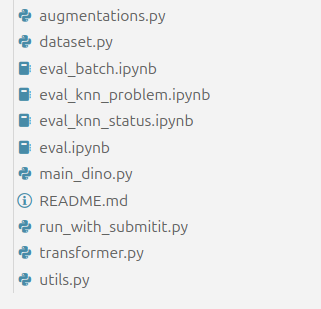
\includegraphics[width=0.6\textwidth]{project_arc.png}
    \caption{Архитектура проекта}
    \label{fig:project_arc}
\end{figure}
\par На рисунке \ref{fig:project_arc} изображена архитектура проекта. Здесь для вызова обучения необходимо запустить файл main\_dino.py, с необходимыми аргументами.
\par Перечень основных аргументов
\begin{itemize}
    \item arch -- название архитектуры, которая будет использована для создания модели, изначально выбран t\_tiny.
    \item token\_slicer -- метод по отделения участков. Изначально стоит Tokens -- разделение на участки по токенам.
    \item max\_token\_count -- максимальное число токенов, в использованном токенизаторе это значение равняется 65536.
    \item out\_dim -- размерность пространства выхода Dino head. Изначально равно 65000.
    \item use\_fp16 -- использовать ли float 16 во время обучения или нет. Изначально флаг равен Истине.
    \item batch\_size\_per\_gpu -- количество примеров которые будут загружены на одной видеокарте. Изначально стоит 16.
    \item epochs -- количество эпох обучения. Изначально равно 100.
    \item local\_crops\_number -- количество локальных участков на одно наблюдение. Изначально равно 8.
\end{itemize}
\par Для запуска был использован персональный компьютер с ОС Ubuntu, GPU Nvidia 3090 с 16гб видеопамяти, и 256 гигабайтами оперативной памяти. При этом, со всеми выставленными настройками было занято 14 из 16 гигабайт видеопамяти.
\par Весь процесс обучения занял 25 часов. Результатом работы был файл checkpoint.pth, в котором находились веса модели учителя и ученика, а так же данные из конфигурации процесса обучения.
\end{document}